\documentclass[tikz,border=10pt]{standalone}
\usetikzlibrary{positioning, arrows.meta, calc, babel, fit, backgrounds}
\usepackage[utf8]{inputenc}
\usepackage[T1]{fontenc}
\usepackage{lmodern}
\usepackage[english]{babel}
\usepackage{amsmath, amssymb, bm}

\begin{document}
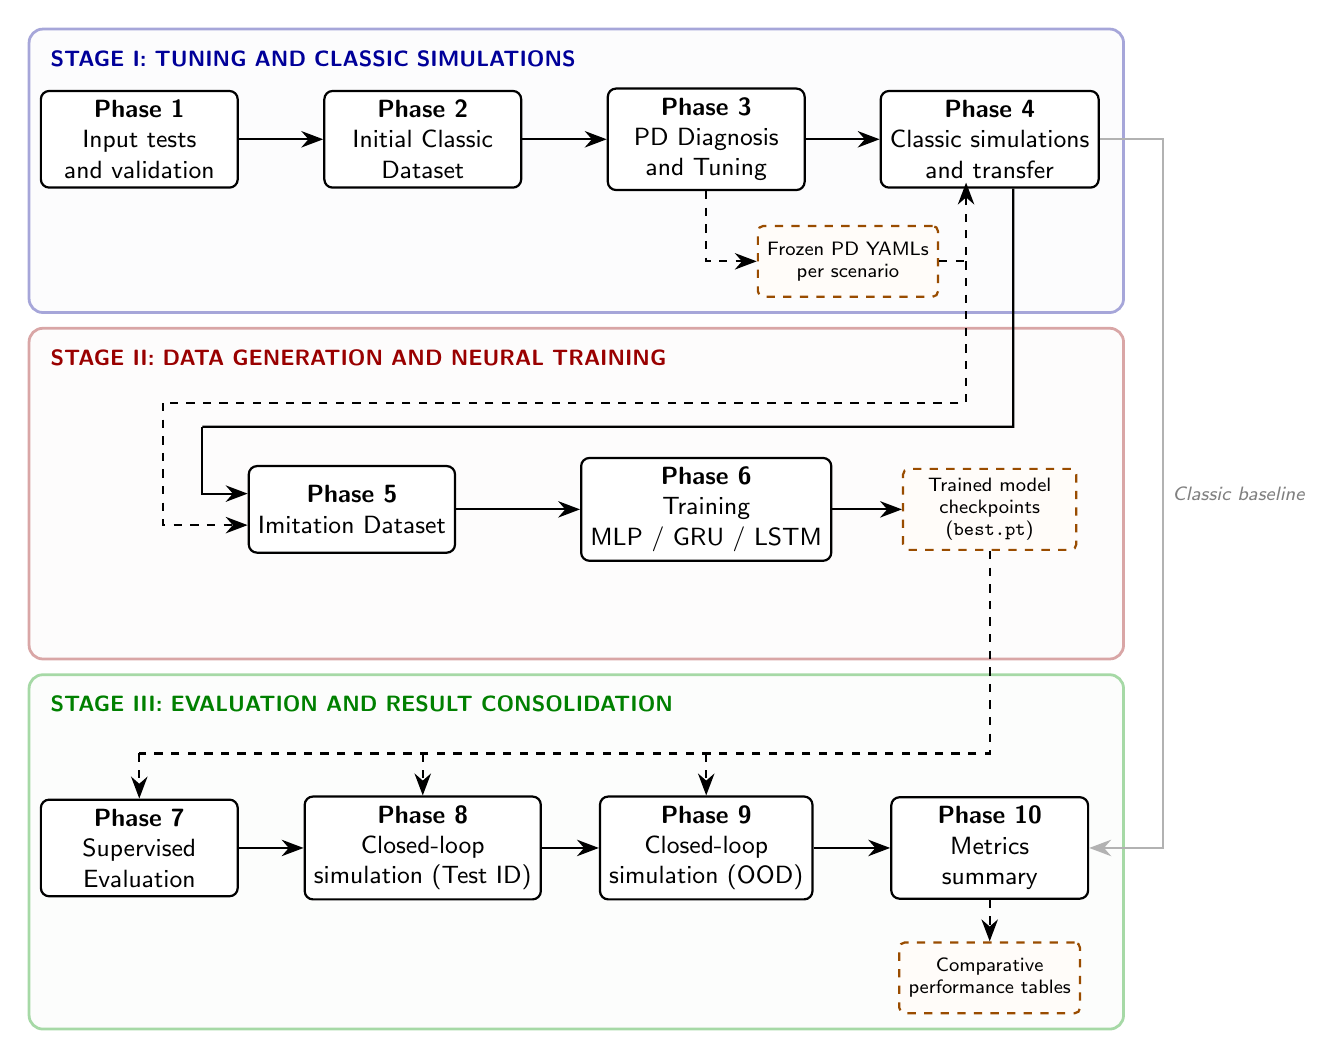
\begin{tikzpicture}[
  align=center,
  font=\sffamily\small,
  % Estilos de bloques
  phasebox/.style={draw, rectangle, rounded corners=3pt, minimum width=2.5cm, minimum height=1.1cm, thick, fill=white},
  artbox/.style={draw, rectangle, dashed, rounded corners=2pt, minimum width=2.2cm, minimum height=0.9cm, fill=yellow!8!orange!2!white, draw=orange!60!black, font=\sffamily\scriptsize, thick},
  groupbox/.style={draw, rectangle, rounded corners=5pt, line width=1.0pt},
  % Estilos de flechas
  line/.style={draw, -{Stealth[scale=1.2]}, thick},
  dashline/.style={draw, -{Stealth[scale=1.2]}, thick, dashed},
  dashseg/.style={draw, thick, dashed}
]

  % ==========================================
  % ROW 1: STAGE I (y = 0.0)
  % ==========================================
  \node[phasebox] (f1) at (0,0) {\textbf{Phase 1}\\Input tests\\ and validation};
  \node[phasebox] (f2) at (3.6,0) {\textbf{Phase 2}\\Initial Classic\\Dataset};
  \node[phasebox] (f3) at (7.2,0) {\textbf{Phase 3}\\PD Diagnosis\\and Tuning};
  \node[phasebox] (f4) at (10.8,0) {\textbf{Phase 4}\\Classic simulations\\and transfer};

  \draw[line] (f1) -- (f2);
  \draw[line] (f2) -- (f3);
  \draw[line] (f3) -- (f4);

  % Frozen PIDs YAML artifact
  \node[artbox] (art_pids) at (9.0,-1.55) {Frozen PD YAMLs\\per scenario};
  
  \draw[dashline] (f3.south) |- (art_pids.west);

  % ==========================================
  % ROW 2: STAGE II (y = -4.7)
  % ==========================================
  \node[phasebox] (f5) at (2.7,-4.7) {\textbf{Phase 5}\\Imitation Dataset};
  \node[phasebox] (f6) at (7.2,-4.7) {\textbf{Phase 6}\\Training\\MLP / GRU / LSTM};
  \node[artbox] (art_weights) at (10.8,-4.7) {Trained model\\checkpoints\\(\texttt{best.pt})};

  % Inputs from Stage I to Phase 5
  \coordinate (in_cont) at (0.8,-3.65);
  \coordinate (in_dash) at (0.3,-3.35);
  
  % Connection of YAML (art_pids) to Phase 4 (input at X=10.5)
  \draw[dashline] (art_pids.east) -- (10.5,-1.55) -- (10.5,-0.55);

  % Continuous data channel
  \draw[thick] ($(f4.south)+(0.3,0)$) -- (11.1,-3.65) -- (in_cont);
  \draw[line] (in_cont) |- ($(f5.west)+(0,+0.2)$);

  % Discontinuous parameter channel
  \draw[thick, dashed] (10.5,-1.55) -- (10.5,-3.35) -- (in_dash);
  \draw[dashline] (in_dash) |- ($(f5.west)+(0,-0.2)$);

  % Direct connection F5 to F6
  \draw[line] (f5.east) -- (f6.west);
  \draw[line] (f6.east) -- (art_weights.west);

  % ==========================================
  % ROW 3: STAGE III (y = -9.0)
  % ==========================================
  \node[phasebox] (f7) at (0,-9.0) {\textbf{Phase 7}\\Supervised\\Evaluation};
  \node[phasebox] (f8) at (3.6,-9.0) {\textbf{Phase 8}\\Closed-loop\\simulation (Test ID)};
  \node[phasebox] (f9) at (7.2,-9.0) {\textbf{Phase 9}\\Closed-loop\\simulation (OOD)};
  \node[phasebox] (f10) at (10.8,-9.0) {\textbf{Phase 10}\\Metrics\\summary};
  \node[artbox] (art_latex) at (10.8,-10.65) {Comparative\\performance tables};

  % Checkpoint bus
  \draw[thick, dashed] (art_weights.south) -- (10.8,-7.8) -- (0,-7.8);
  \draw[dashline] (0,-7.8) -- (f7.north);
  \draw[dashline] (3.6,-7.8) -- (f8.north);
  \draw[dashline] (7.2,-7.8) -- (f9.north);

  \draw[line] (f7) -- (f8);
  \draw[line] (f8) -- (f9);
  \draw[line] (f9) -- (f10);
  \draw[dashline] (f10.south) -- (art_latex.north);

  % ==========================================
  % CLASSIC BASELINE
  % ==========================================
  \draw[line, draw=black!30] (f4.east) -- (13.0,0) -- (13.0,-9.0) -- (f10.east);
  \node[right, font=\sffamily\scriptsize\itshape, text=black!50] at (13.0,-4.5) {Classic baseline};

  % ==========================================
  % BACKGROUND LAYER
  % ==========================================
  \begin{scope}[on background layer]
    % Stage I Panel
    \draw[groupbox, fill=blue!5!gray!2, draw=blue!40!gray!50] (-1.4, 1.4) rectangle (12.5, -2.2);
    % Stage II Panel
    \draw[groupbox, fill=red!5!gray!2, draw=red!40!gray!50] (-1.4, -2.4) rectangle (12.5, -6.6);
    % Stage III Panel
    \draw[groupbox, fill=green!5!gray!2, draw=green!40!gray!50] (-1.4, -6.8) rectangle (12.5, -11.3);
  \end{scope}

  % Stage titles
  \node[anchor=north west, font=\sffamily\bfseries\footnotesize, color=blue!60!black] at (-1.25, 1.25) {STAGE I: TUNING AND CLASSIC SIMULATIONS};
  \node[anchor=north west, font=\sffamily\bfseries\footnotesize, color=red!60!black] at (-1.25, -2.55) {STAGE II: DATA GENERATION AND NEURAL TRAINING};
  \node[anchor=north west, font=\sffamily\bfseries\footnotesize, color=green!50!black] at (-1.25, -6.95) {STAGE III: EVALUATION AND RESULT CONSOLIDATION};

\end{tikzpicture}
\end{document}
